% !TeX program = xelatex
% 作业一：文本分类实现 —— 实验报告
% 编译：xelatex report.tex （连续两次，以生成目录）
\documentclass[12pt,a4paper]{ctexart}

\usepackage{geometry}
\geometry{left=2.4cm,right=2.4cm,top=2.6cm,bottom=2.6cm}
\usepackage{graphicx}
\graphicspath{{report/figs/}{figs/}}
\usepackage{booktabs}
\usepackage{amsmath,amssymb}
\usepackage[hidelinks]{hyperref}

\setlength{\emergencystretch}{3em}

\newcommand{\fpath}[1]{\texttt{#1}}
\newcommand{\best}[1]{\textbf{#1}}

\title{\bfseries 作业一：文本分类实现\\[6pt]
\large Bag of Words、Word2Vec 与 BERT 三种文本表示方法的对比研究}
\author{姓名：郝普瑞 \quad 学号：2310412}
\date{2026 年 10 月 9 日}

\begin{document}
\maketitle

\begin{abstract}
\noindent
本报告在 NYT 三分类新闻数据集上，系统比较了三类文本表示方法：
基于词袋的离散表示（Binary BoW / Word Frequency）、
基于词向量的稠密表示（预训练 GloVe、自训练 Word2Vec）、
以及基于预训练语言模型的上下文表示（BERT-base-uncased 微调）。
所有实验共用同一份 80\%/10\%/10\% 数据划分，分类器统一为 Logistic Regression
（BERT 除外），评价指标统一为 Accuracy 与 Macro-F1。

主要发现：（1）\textbf{词袋表示在该数据集上异常强}，词频词袋的 Test Macro-F1 达 0.9542，
优于随机初始化的词向量平均；（2）\textbf{词向量的价值主要体现在压缩比}——
100 维 GloVe 追平了 53146 维的 Binary BoW（0.9471 vs 0.9468），
维度压缩约 500 倍而性能几乎不变；（3）\textbf{BERT 微调取得最优结果但优势有限}——
4 次独立运行的 Test Macro-F1 为 $0.9597 \pm 0.0033$，
平均仅比最强词袋高 0.0055，且受 GPU 浮点非确定性影响，单次结果不可复现；
（4）错误高度集中在 business $\leftrightarrow$ politics 之间（占全部错误的 75\%），
而 sports 类的错分率仅 0.35\%。
\end{abstract}

\tableofcontents
\newpage

% ============================================================
\section{实验目的与任务概述}

本实验旨在理解并比较不同文本表示方法在文本分类任务中的原理与效果，
具体包括四个目标：掌握词袋表示与 Logistic Regression 的基本用法；
掌握 Word2Vec / GloVe 词向量的获取与使用；
熟悉 BERT 类预训练语言模型的微调流程；
并能够用 Accuracy 与 Macro-F1 对模型做出评价与横向比较。

作业包含三个任务：

\begin{itemize}
  \item \textbf{Task 1（Bag of Words）}：用 Binary BoW 与 Word Frequency 两种词袋表示，
        分别训练 Logistic Regression 分类器；
  \item \textbf{Task 2（Word2Vec）}：统一使用 100 维词向量，
        分别来自预训练 GloVe、AG News 自训练 Word2Vec、NYT 自训练 Word2Vec，
        文档向量取文档内有效词向量的平均，再用 Logistic Regression 分类；
  \item \textbf{Task 3（预训练语言模型）}：微调 \fpath{google-bert/bert-base-uncased}，
        设置 \fpath{max\_length = 64}、训练 3 epochs。
\end{itemize}

表~\ref{tab:compliance} 对照列出作业的硬性要求与本实验的实现方式。

\begin{table}[htbp]
\centering
\small
\caption{作业要求与本实验实现的对照}
\label{tab:compliance}
\begin{tabular}{p{5.6cm}p{9.4cm}}
\toprule
作业要求 & 本实验实现 \\
\midrule
Task 1：两种 BoW 表示 + LR，报告 Acc 与 Macro-F1
  & Binary BoW 与 Word Frequency 各一组，另加两组 \fpath{class\_weight=balanced} 对照 \\
Task 2：统一 100 维词向量，文档向量为词向量平均，分类器为 LR
  & GloVe-100 / Word2Vec(AG News)-100 / Word2Vec(NYT)-100 三组，
    $e(d)=\frac{1}{n}\sum_{i=1}^{n}e(w_i)$，LR 分类 \\
Task 3：\fpath{bert-base-uncased}，\fpath{max\_length=64}，3 epochs
  & 该模型、该长度、该轮数，严格遵守 \\
NYT 随机打乱后按 80\%/10\%/10\% 划分，所有实验使用同一划分
  & 由 \fpath{code/step0\_split.py} 一次性生成并落盘，
    \fpath{seed=42}，六个实验共用 \fpath{data/\{train,val,test\}.csv} \\
统一在 NYT Test Set 上评价，报告 Accuracy 与 Macro-F1
  & 全部结果均在 1145 条 Test 样本上给出，指标同时报告 \\
\bottomrule
\end{tabular}
\end{table}

% ============================================================
\section{数据集与统一实验设置}

\subsection{数据集与统计}

实验主数据集为 NYT 新闻数据（\fpath{HW-1/nyt.csv}，字段为 \fpath{text} 与 \fpath{label}），
辅助数据集为 AG News（\fpath{HW-1/ag.csv}，仅提供 \fpath{text}，用于训练 Word2Vec）。
清洗方式为去除空值并按 \fpath{text} 去重。统计结果见表~\ref{tab:dataset}。

\begin{table}[htbp]
\centering
\small
\caption{NYT 数据集统计（清洗后）}
\label{tab:dataset}
\begin{tabular}{lll}
\toprule
项目 & 值 & 说明 \\
\midrule
总样本数 & 11447 & — \\
类别数 & 3 & business / politics / sports \\
sports & 8597（\best{75.1\%}） & 绝对多数类 \\
politics & 1433（12.5\%） & — \\
business & 1417（12.4\%） & — \\
平均文本长度 & 637.1 词 & 按空格切分粗略统计 \\
平均 subword token 数 & \best{834.2} & 中位数 872 / P90 1239 / 最长 6775 \\
超过 64 token 的文档占比 & \best{99.96\%} & 截断后平均保留 \best{7.67\%} \\
Training / Validation / Test & 9157 / 1145 / 1145 & 80\% / 10\% / 10\% \\
\bottomrule
\end{tabular}
\end{table}

有两个必须在报告中讨论的数据特点：

\textbf{（1）类别严重不均衡。}
sports 占 75.1\%，因此 Accuracy 存在约 75\% 的``地板''：
一个永远输出 sports 的平凡基线即可获得 0.7511 的 Accuracy（实测，见表~\ref{tab:main}）。
这直接说明\textbf{必须同时考察 Macro-F1}——该基线的 Macro-F1 仅为 0.2860。
这也是作业要求同时报告两个指标的动机。

\textbf{（2）文本极长，而作业规定 BERT 的 \fpath{max\_length=64}。}
实测平均 834.2 个 subword token（中位数 872，P90 1239，最长 6775），
\textbf{99.96\% 的文档会被截断}，截断后平均仅保留 \textbf{7.67\%} 的 token。
即 BERT 只能看到每篇文档开头约 7.7\% 的内容。
该参数是作业硬性规定，必须遵守，但需在第~\ref{sec:bert-trunc} 节量化其影响。

\subsection{数据划分}

按作业要求，先对 NYT 数据集做随机打乱，再按 80\%/10\%/10\% 划分为
Training / Validation / Test（\fpath{seed=42}，且按类别分层抽样以保证三份数据的类别比例一致）。
划分结果由 \fpath{code/step0\_split.py --stratify} 落盘到 \fpath{data/}，
后续所有任务均读取这三份文件，
从而\textbf{保证不同方法之间的可比性}——这是跨任务比较的前提。

需要说明的是：\textbf{词表与文档向量统计均只在训练集上拟合}。
Task 1 的词表仅用训练集 \fpath{fit}，val/test 只做 \fpath{transform}；
Task 2 中 NYT 自训练 Word2Vec 也只使用训练集的 9157 篇文本，
以避免验证/测试集的信息泄漏。

\subsection{评价指标}

\textbf{Accuracy} 为分类正确的样本数占全部测试样本的比例：

\begin{equation}
\mathrm{Accuracy} = \frac{1}{N}\sum_{i=1}^{N}\mathbb{1}\left[\hat{y}_i = y_i\right]
\end{equation}

\textbf{Macro-F1} 先对每个类别分别计算 F1，再做算术平均（各类权重相同）：

\begin{equation}
\mathrm{Macro\text{-}F1} = \frac{1}{C}\sum_{c=1}^{C} \frac{2P_c R_c}{P_c + R_c},
\qquad
P_c=\frac{TP_c}{TP_c+FP_c},\quad
R_c=\frac{TP_c}{TP_c+FN_c}
\end{equation}

其中 $C=3$ 为类别数。由于各类权重相同，Macro-F1 对少数类的表现更敏感，
在类别不均衡的数据上比 Accuracy 更能反映真实分类能力。

\subsection{实验环境}

\begin{table}[htbp]
\centering
\small
\caption{实验环境}
\label{tab:env}
\begin{tabular}{ll}
\toprule
项目 & 版本 / 配置 \\
\midrule
操作系统 & Windows \\
GPU & NVIDIA GeForce RTX 4060 Laptop GPU（8\,GB 显存） \\
显卡驱动 & 566.26（支持 CUDA $\le$ 12.7） \\
Python & 3.11.17（conda 环境） \\
torch & 2.6.0+cu124 \\
transformers & 5.19.0 \\
datasets / accelerate & 5.1.0 / 1.15.0 \\
gensim & 4.4.0 \\
scikit-learn & 1.9.1 \\
numpy / pandas & 2.4.6 / 3.0.6 \\
nltk & 3.10.3 \\
\bottomrule
\end{tabular}
\end{table}

\fpath{torch.cuda.is\_available()} 验证结果为 \fpath{True}，
BERT 训练使用 bf16 混合精度。

% ============================================================
\section{Task 1：基于词袋表示的文本分类}

\subsection{方法原理}

设训练语料构建的词表大小为 $|V|$，则每篇文档被表示为 $|V|$ 维向量。

\textbf{Binary Bag of Words} 只记录词是否出现：

\begin{equation}
x_i =
\begin{cases}
1, & \text{词表中第 } i \text{ 个词出现在文档中}\\
0, & \text{否则}
\end{cases}
\end{equation}

\textbf{Word Frequency} 记录词在当前文档中的出现次数：

\begin{equation}
x = (c_1, c_2, \ldots, c_{|V|}), \qquad c_i = \text{第 } i \text{ 个词的出现次数}
\end{equation}

两种表示得到的高维稀疏向量直接作为 Logistic Regression 的输入特征。

\subsection{实现细节}

\begin{itemize}
  \item \textbf{分词}：统一使用小写化 + nltk \fpath{word\_tokenize}（\fpath{code/common.py} 中的 \fpath{tokenize}），
        保证三个任务的分词口径一致；
  \item \textbf{词表}：\fpath{CountVectorizer}，设置 \fpath{min\_df=2} 丢弃出现次数少于 2 的极低频词，
        且\textbf{仅在训练集上 \fpath{fit}}；
  \item \textbf{分类器}：\fpath{LogisticRegression(max\_iter=1000, C=1.0)}，默认 lbfgs 求解器；
  \item \textbf{对照实验}：额外运行 \fpath{class\_weight="balanced"} 的两组，
        考察类别不均衡的影响；
  \item \textbf{基线}：同时打印``永远预测多数类''的平凡基线，作为参照系。
\end{itemize}

\subsection{实验结果}

\begin{table}[htbp]
\centering
\footnotesize
\caption{Task 1 结果（NYT Test Set，1145 条）}
\label{tab:task1}
\begin{tabular}{llccccc}
\toprule
方法 & 词表 $|V|$ & Val Acc & Val Macro-F1 & Test Acc & Test Macro-F1 \\
\midrule
多数类基线 & — & — & — & 0.7511 & 0.2860 \\
Binary BoW + LR & 53146 & 0.9773 & 0.9436 & 0.9790 & 0.9468 \\
Word Frequency + LR & 53146 & 0.9764 & 0.9449 & \best{0.9825} & \best{0.9542} \\
Binary BoW + LR（balanced） & 53146 & 0.9808 & 0.9514 & 0.9790 & 0.9479 \\
Word Frequency + LR（balanced） & 53146 & 0.9790 & 0.9485 & 0.9808 & 0.9506 \\
\bottomrule
\end{tabular}
\end{table}

图~\ref{fig:t1-binary} 与图~\ref{fig:t1-freq} 为两组主实验的终端输出，
图~\ref{fig:t1-bin-bal} 与图~\ref{fig:t1-freq-bal} 为两组类别权重对照实验的输出。

\begin{figure}[htbp]
  \centering
  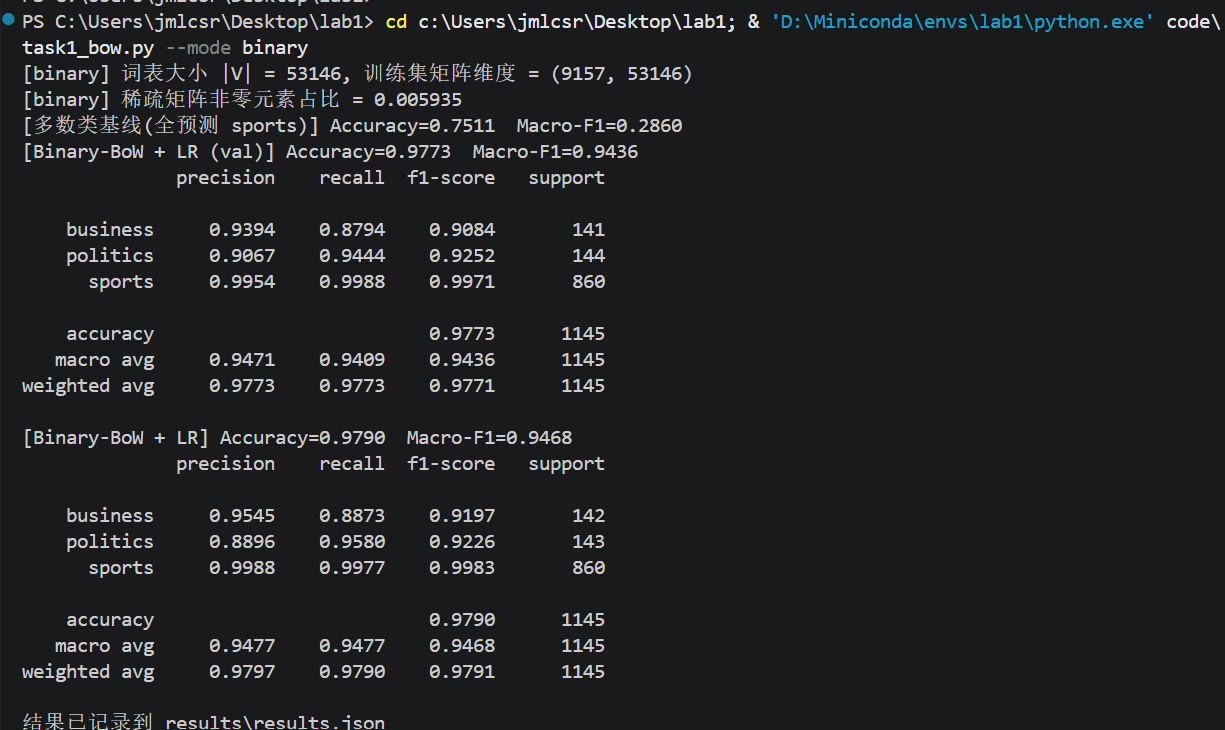
\includegraphics[width=0.95\linewidth]{t1_01_binary.png}
  \caption{Binary Bag of Words + LR 的运行输出。
  可见词表规模 $|V|=53146$、稀疏矩阵非零元素占比 0.5935\%、
  多数类基线 Acc 0.7511 / Macro-F1 0.2860，
  最终 Test Acc 0.9790 / Macro-F1 0.9468。}
  \label{fig:t1-binary}
\end{figure}

\begin{figure}[htbp]
  \centering
  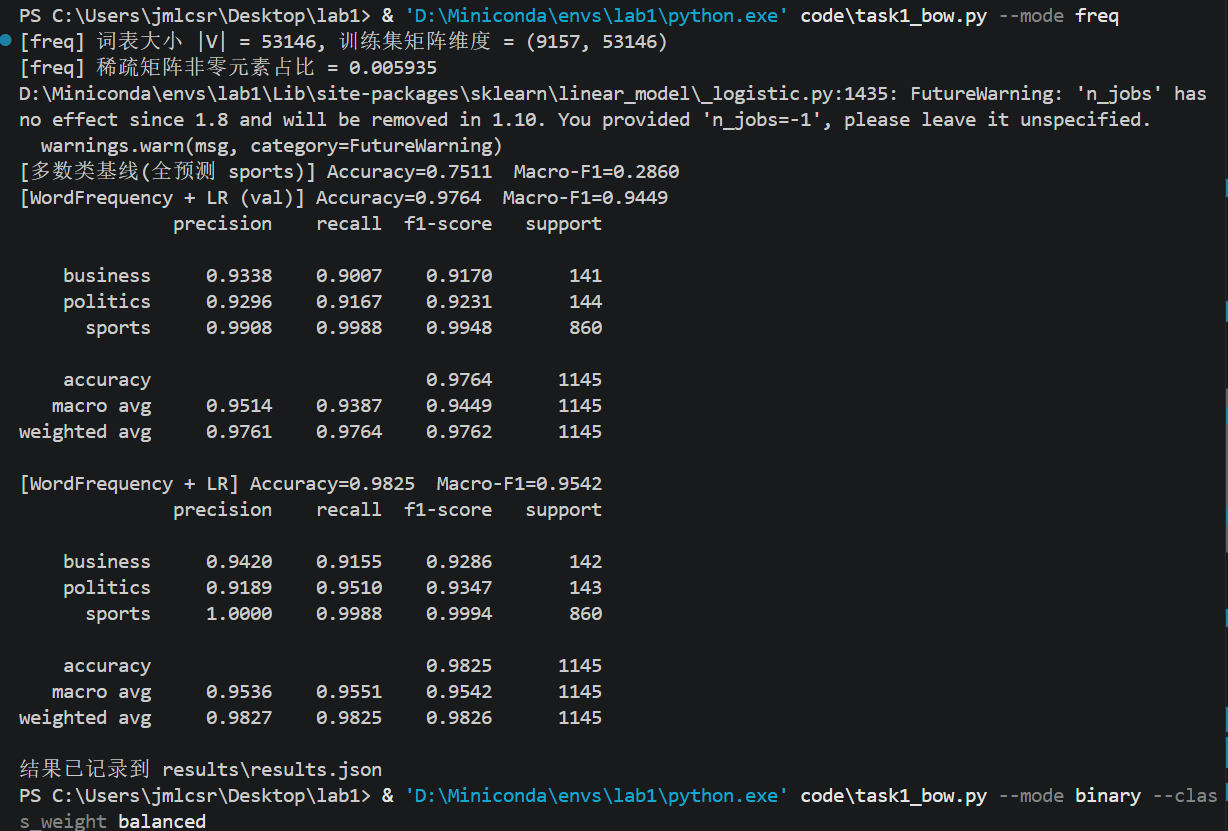
\includegraphics[width=0.95\linewidth]{t1_03_freq.png}
  \caption{Word Frequency + LR 的运行输出。
  词表规模与 Binary 完全相同（53146），
  最终 Test Acc 0.9825 / Macro-F1 0.9542，优于二值表示。}
  \label{fig:t1-freq}
\end{figure}

\begin{figure}[htbp]
  \centering
  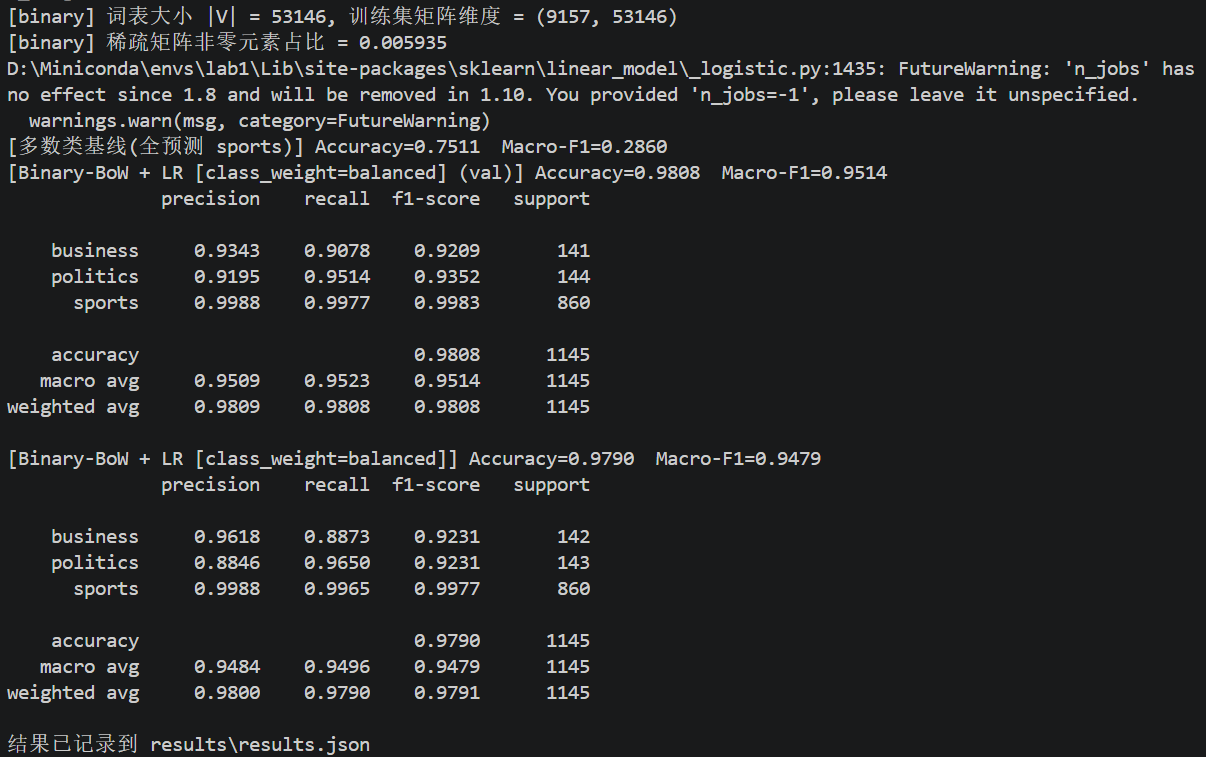
\includegraphics[width=0.95\linewidth]{t1_04_binary_balanced.png}
  \caption{Binary BoW + LR（\fpath{class\_weight="balanced"}）的输出。
  Test Acc 0.9790 / Macro-F1 0.9479，与不加权基本持平。}
  \label{fig:t1-bin-bal}
\end{figure}

\begin{figure}[htbp]
  \centering
  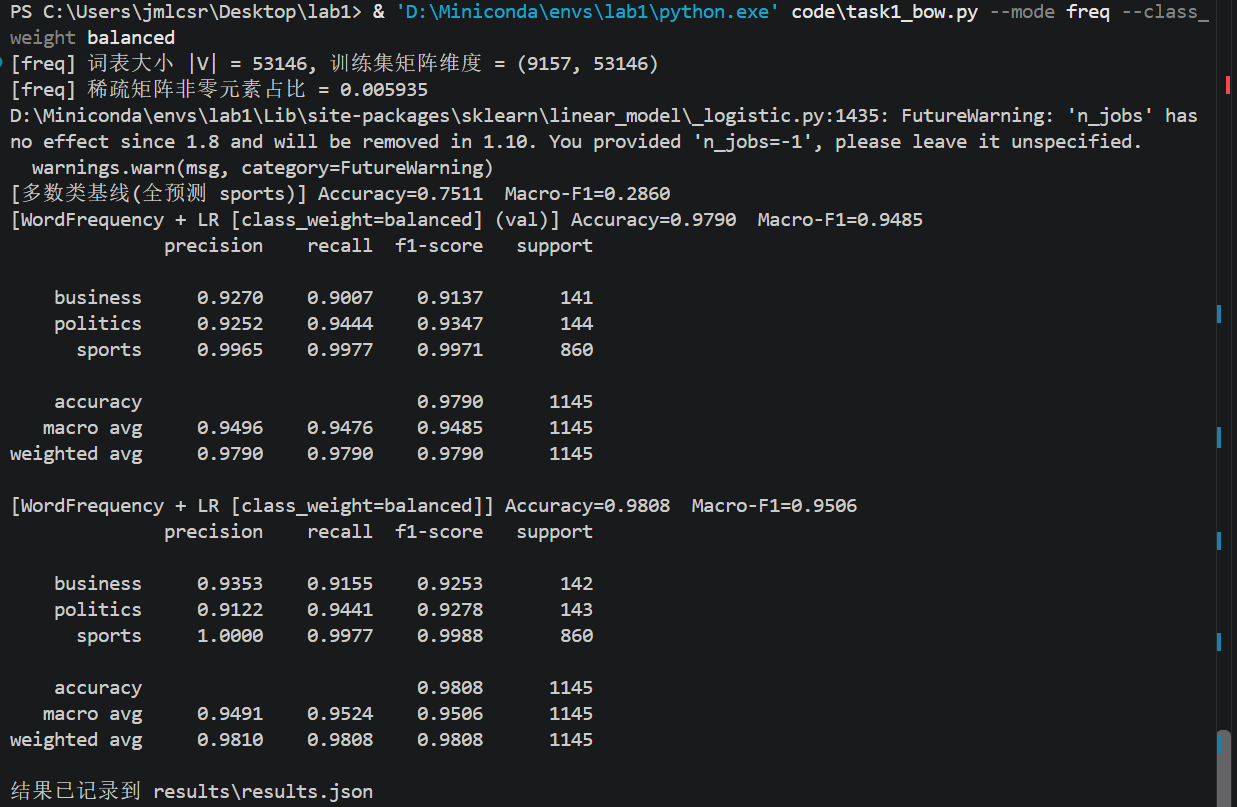
\includegraphics[width=0.95\linewidth]{t1_05_freq_balanced.png}
  \caption{Word Frequency + LR（\fpath{class\_weight="balanced"}）的输出。
  Test Acc 0.9808 / Macro-F1 0.9506，反而略低于不加权版本。}
  \label{fig:t1-freq-bal}
\end{figure}

\subsection{结果分析}

\textbf{（1）两种词袋都极强，且远好于平凡基线。}
Test Accuracy 在 0.979$\sim$0.983 之间，Macro-F1 在 0.947$\sim$0.954 之间。
相比多数类基线的 Macro-F1 0.2860，提升约 \textbf{+0.67}，
说明模型确实学到了区分性特征，而不是靠猜多数类。

\textbf{（2）Word Frequency 优于 Binary BoW。}
Test Macro-F1 为 0.9542 vs 0.9468（+0.0074），
Accuracy 为 0.9825 vs 0.9790（+0.0035）。
两组实验的维度完全相同（$|V|=53146$），
唯一的差别就是\textbf{是否保留词频}，
因此该差异可归因于词频携带了``强度''信息——
某类新闻的特征词往往在文中反复出现。

\textbf{（3）\fpath{class\_weight="balanced"} 没有系统性收益。}
Binary 从 0.9468 变为 0.9479（+0.0011），
Frequency 从 0.9542 变为 0.9506（$-0.0036$），
两者都在随机波动范围内。
原因在于：该数据集虽然类别不均衡，但\textbf{类别可分性极强}
（sports 的特征词极为显著），默认 LR 已能把少数类学好；
\fpath{balanced} 只是把少数类 recall 拉高、precision 拉低，Macro-F1 因此打平。

\textbf{（4）高维稀疏的具体形态。}
词表共 53146 个词，训练矩阵为 $9157 \times 53146$（约 4.87 亿个元素），
非零元素仅占 \textbf{0.5935\%}（稀疏度 99.41\%），
等价于每篇文档平均只用到约 315 个不同的词（而全文平均 637 词）。
这是``词表大、单篇用词集中''的直接结果。
需要说明的是，非零占比只是表示的形态描述，\textbf{不是评价指标}。

\textbf{（5）val 与 test 高度一致}（如 Binary：0.9436 vs 0.9468），
没有明显过拟合，test 略优于 val 属于抽样波动。

\textbf{（6）该实验是确定性的。}
在去掉 sklearn 已忽略的 \fpath{n\_jobs} 参数后重跑 \fpath{--mode binary}，
输出与修改前\textbf{逐位完全一致}（Val 0.9773/0.9436、Test 0.9790/0.9468，
$|V|$ 与非零占比亦相同）。这说明 Task 1 无随机成分
（\fpath{CountVectorizer} 是确定性的，\fpath{lbfgs} 求解器无随机初始化），
\textbf{重复运行只会得到完全相同的结果}，因此无需多次实验。

% ============================================================
\section{Task 2：基于词向量的文本分类}

\subsection{方法原理}

统一使用 100 维词向量。对一篇包含 $n$ 个有效词（能在词向量表中查到）的文档，
其文档向量为所有有效词向量的平均：

\begin{equation}
e(d) = \frac{1}{n}\sum_{i=1}^{n} e(w_i)
\end{equation}

该表示把任意长度的文档压缩为固定 100 维的稠密向量，
再交给 Logistic Regression 分类。
若文档中不存在任何有效词，则退回零向量（本实验中该情况出现 0 次）。

三组实验的唯一变量是\textbf{词向量的来源}：
预训练 GloVe（60 亿词语料）、AG News 自训练、NYT 自训练。

\subsection{三组实验设置}

\begin{itemize}
  \item \textbf{GloVe-100}：官方 \fpath{glove.6B.100d.txt}（347,117,594 字节，已核对与官方一致），
        词表 400,001 词；
  \item \textbf{Word2Vec(AG News)}：在 AG News 的 90,000 条文本上训练，
        语料共 4,051,013 词（平均每篇仅 45 词），词表 25,376；
  \item \textbf{Word2Vec(NYT)}：\textbf{仅用训练集}的 9,157 篇文本训练（避免 val/test 信息泄漏），
        语料共 6,676,990 词（平均每篇 729 词），词表 31,579。
\end{itemize}

Word2Vec 训练超参数统一为 \fpath{vector\_size=100}、\fpath{window=5}、\fpath{min\_count=5}、
\fpath{sg=1}、\fpath{negative=5}、\fpath{epochs=10}、\fpath{seed=42}
（Skip-gram + 负采样）。分类器统一为 \fpath{LogisticRegression(max\_iter=2000)}。

\subsection{实验结果}

\begin{table}[htbp]
\centering
\footnotesize
\caption{Task 2 结果（NYT Test Set，1145 条）}
\label{tab:task2}
\begin{tabular}{llcccc}
\toprule
词向量来源 & 训练语料 & 词表 & 词覆盖率(test) & Test Acc & Test Macro-F1 \\
\midrule
GloVe-100（预训练） & 60 亿词 & 400001 & \best{98.06\%} & 0.9782 & \best{0.9471} \\
Word2Vec(NYT)-100 & 6.68M 词（同领域） & 31579 & 97.58\% & 0.9712 & 0.9308 \\
Word2Vec(AG News)-100 & 4.05M 词（跨领域） & 25376 & 94.32\% & 0.9686 & 0.9227 \\
\bottomrule
\end{tabular}
\end{table}

图~\ref{fig:t2-glove}、图~\ref{fig:t2-ag}、图~\ref{fig:t2-nyt}
分别为三组实验的终端输出。

\begin{figure}[htbp]
  \centering
  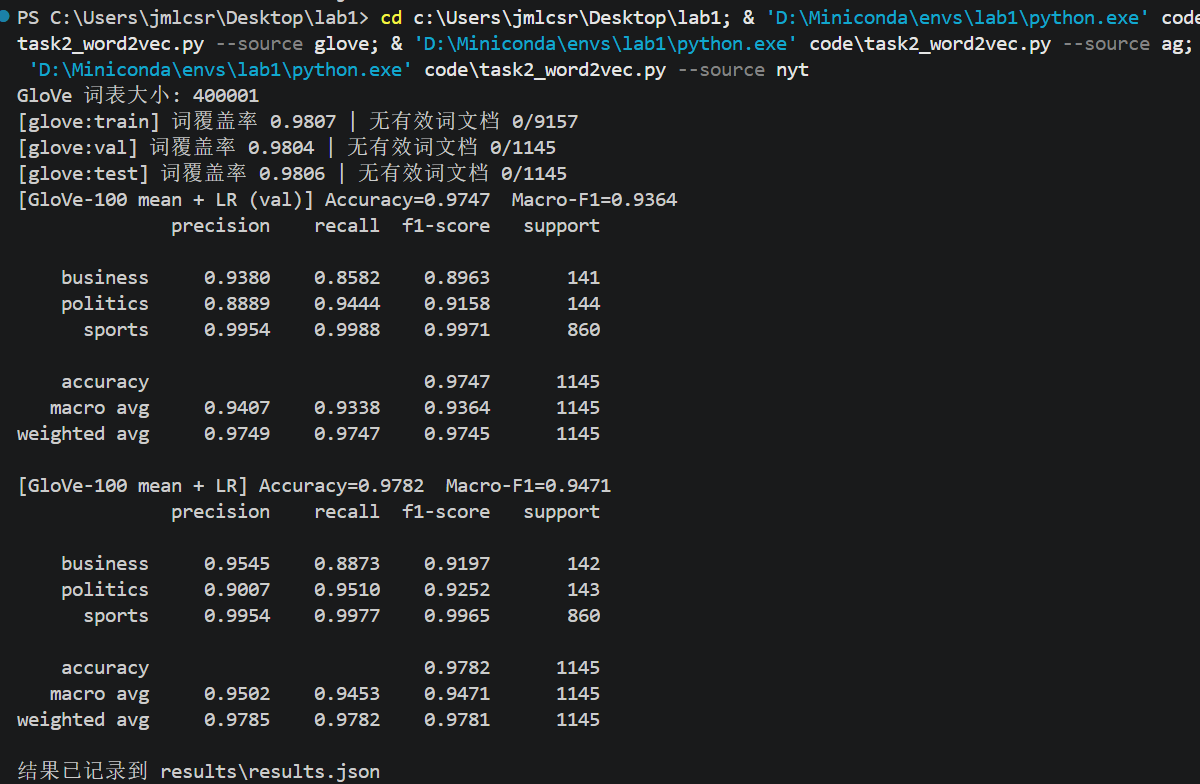
\includegraphics[width=0.95\linewidth]{t2_01_glove.png}
  \caption{预训练 GloVe-100 平均词向量 + LR 的输出。
  词表 400,001，词覆盖率 98.07\%，Test Acc 0.9782 / Macro-F1 0.9471。}
  \label{fig:t2-glove}
\end{figure}

\begin{figure}[htbp]
  \centering
  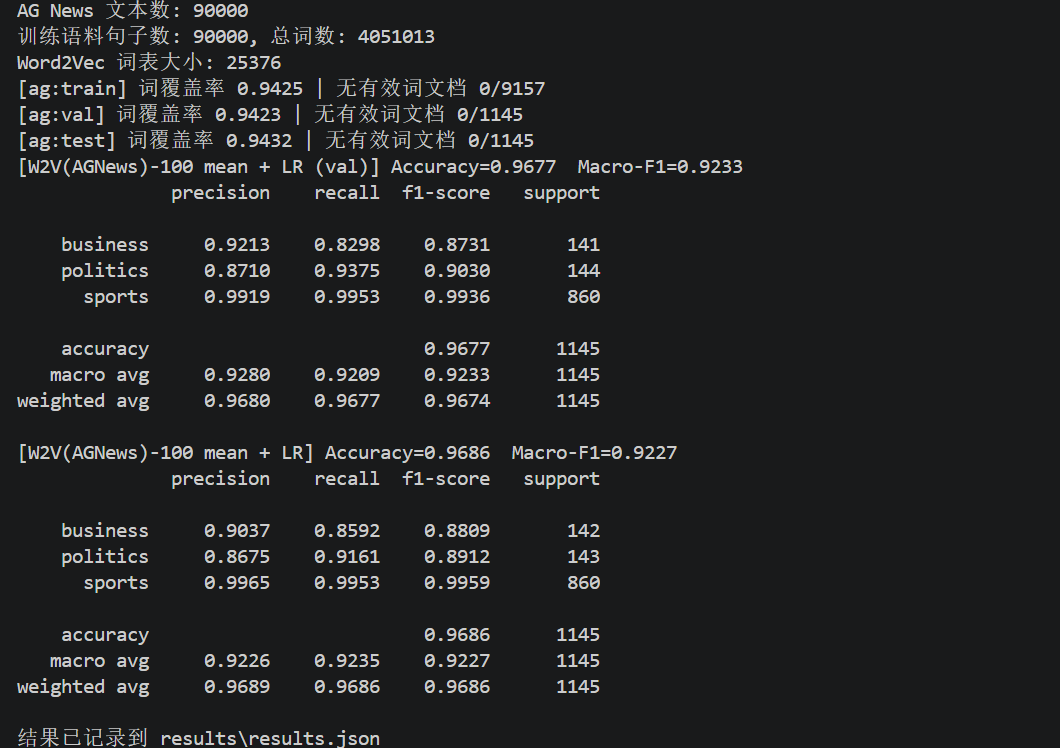
\includegraphics[width=0.95\linewidth]{t2_02_agnews.png}
  \caption{Word2Vec(AG News)-100 平均词向量 + LR 的输出。
  训练语料 4,051,013 词，词表 25,376，词覆盖率 94.32\%，
  Test Acc 0.9686 / Macro-F1 0.9227。}
  \label{fig:t2-ag}
\end{figure}

\begin{figure}[htbp]
  \centering
  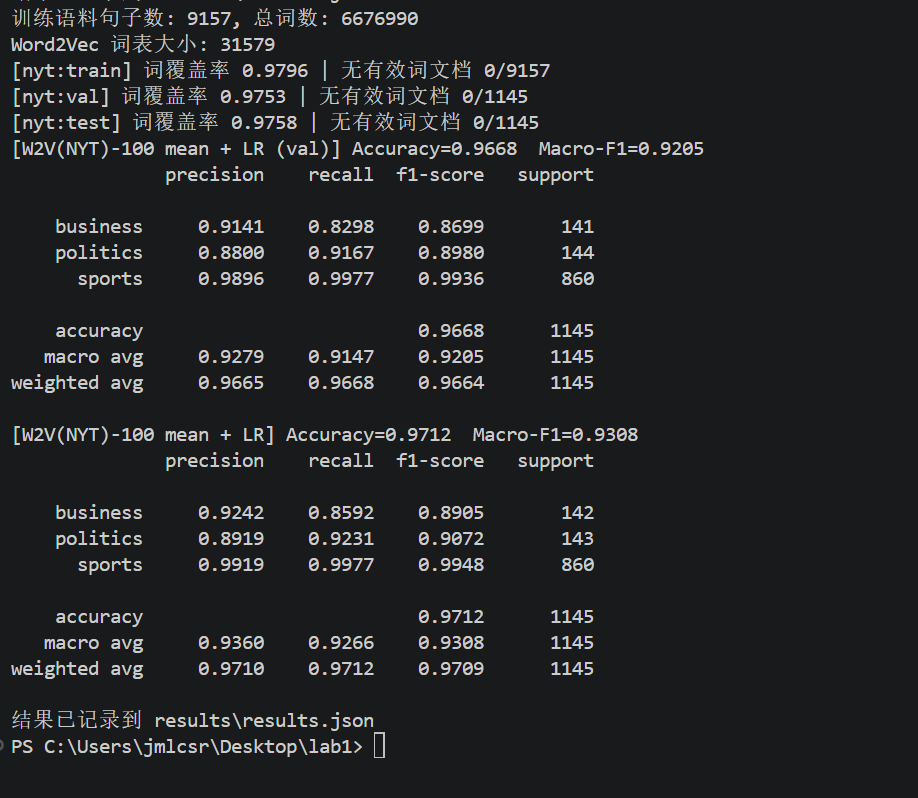
\includegraphics[width=0.95\linewidth]{t2_03_nyt.png}
  \caption{Word2Vec(NYT)-100 平均词向量 + LR 的输出。
  仅用训练集 9,157 篇文本训练，词表 31,579，词覆盖率 97.58\%，
  Test Acc 0.9712 / Macro-F1 0.9308。}
  \label{fig:t2-nyt}
\end{figure}

\subsection{结果分析}

\textbf{（1）核心规律：词覆盖率与 Macro-F1 完全同序。}

\begin{equation*}
\text{覆盖率：}\ 98.06\% > 97.58\% > 94.32\%
\qquad\Longleftrightarrow\qquad
\text{Macro-F1：}\ 0.9471 > 0.9308 > 0.9227
\end{equation*}

三组实验的唯一差别是词向量来源，因此覆盖率能够完整解释性能排序。
其机理是：覆盖率低 $\Rightarrow$ 更多词查不到词向量
$\Rightarrow$ 文档平均向量被``稀释''（分母 $n$ 变小但有效信息更少）、判别信息减少。
需要说明的是，三组的``无有效词文档数''均为 0，
即不存在被喂入全零向量的文档，性能差异来自覆盖率的精细差别而非极端情形。

\textbf{（2）同领域自训练优于跨领域自训练。}
W2V(NYT) 的 Macro-F1 为 0.9308，高于 W2V(AG News) 的 0.9227（+0.0081），
原因有二：语料与测试集同领域（都是 NYT 新闻），
且覆盖率更高（97.58\% vs 94.32\%）。
AG News 文本极短（平均 45 词），可供模型学习的上下文共现信息也有限。

\textbf{（3）自训练词向量仍明显落后于预训练 GloVe。}
W2V(NYT) 比 GloVe 低 0.0163（0.9308 vs 0.9471）。
决定性因素是\textbf{语料规模的数量级差距}：
自训练语料仅 668 万词，而 GloVe 基于 60 亿词，相差近 900 倍。

\textbf{（4）与 Task 1 的关系（重要）：``压缩比''才是词向量的核心贡献。}
GloVe 以 \textbf{100 维}追平了 \textbf{53146 维}的 Binary BoW
（0.9471 vs 0.9468，仅差 0.0003），
即约 \textbf{500 倍维度压缩而性能几乎无损}——
说明``词向量平均''在\textbf{高维稀疏 $\to$ 低维稠密}的转换上是成功的。
但它并未超越词频词袋（低 0.0071）。
这与数据集特点有关：文本极长（平均 637 词），词袋能无损保留全部词汇信息，
而平均词向量把 637 个词压成 100 维，信息损失较大；
同时平均操作丢弃了语序，``狗咬人''与``人咬狗''不可区分。

% ============================================================
\section{Task 3：基于 BERT 微调的文本分类}

\subsection{方法原理}

BERT 是双向 Transformer 编码器，在大规模语料上通过掩码语言模型等目标预训练，
能够得到\textbf{上下文相关}的词表示。
用于文本分类时，在 \fpath{[CLS]} 位置的输出（经 pooler）之上接一个线性分类头，
然后用下游数据\textbf{微调}整个网络。

与 Task 2 的``平均词向量''相比，其关键差异是：
\begin{itemize}
  \item 表示是\textbf{上下文相关}的，同一个词在不同语境下得到不同向量；
  \item 表示是\textbf{端到端学习}的，不依赖预先固定的词向量表；
  \item 因此不需要手动词表与 OOV 处理，理论上能更好地刻画长距离依赖。
\end{itemize}

\subsection{实验设置}

\begin{table}[htbp]
\centering
\small
\caption{Task 3 超参数}
\label{tab:bert-param}
\begin{tabular}{ll}
\toprule
参数 & 值 \\
\midrule
预训练模型 & \fpath{google-bert/bert-base-uncased} \\
max\_length & \best{64}（作业硬性要求） \\
epochs & \best{3}（作业硬性要求） \\
learning\_rate & 2e-5 \\
batch size & 16（train）/ 32（eval） \\
weight\_decay & 0.01 \\
混合精度 & bf16（RTX 4060 支持） \\
seed & 42 \\
训练步数 & 1719（$9157/16\times3$） \\
单次耗时 & 133.7 $\sim$ 219.8 秒 \\
\bottomrule
\end{tabular}
\end{table}

关于模型加载时的键不匹配：加载 BERT 预训练权重时会报告 7 个 \fpath{UNEXPECTED} 键
（\fpath{cls.predictions.*} 的 MLM 头与 \fpath{cls.seq\_relationship.*} 的 NSP 头，约 62 万参数）
与 2 个 \fpath{MISSING} 键（\fpath{classifier.weight/bias}，仅 2307 个参数）。
这是迁移学习\textbf{预期且必需}的行为：预训练任务的头被丢弃，
新的分类头被随机初始化后由下游数据训练。
若 \fpath{classifier} 不出现 \fpath{MISSING}，反而说明加载了错误的任务头。

\subsection{截断分析}
\label{sec:bert-trunc}

由 \fpath{code/analyze.py} 对全部 11447 篇文档统计得到表~\ref{tab:trunc}。

\begin{table}[htbp]
\centering
\small
\caption{BERT 输入截断统计（\fpath{max\_length=64}，11447 篇）}
\label{tab:trunc}
\begin{tabular}{lc}
\toprule
项目 & 值 \\
\midrule
平均 / 中位数 / P90 / 最长 token 数 & 834.2 / 872 / 1239 / 6775 \\
被截断的文档占比 & \best{99.96\%} \\
平均保留 token 比例 & \best{7.67\%} \\
\bottomrule
\end{tabular}
\end{table}

即 BERT 实际只能看到每篇文档开头约 7.7\% 的内容。
值得注意的是\textbf{中位数（872）大于平均数（834.2）}，
说明 token 长度分布左偏——少数很短的快讯把均值拉低了，
绝大多数文档其实比平均值更长，截断问题比平均值看起来更严重。

图~\ref{fig:analyze} 为该统计脚本的完整输出（下半部分为测试集混淆矩阵，见第~\ref{sec:error} 节）。

\begin{figure}[htbp]
  \centering
  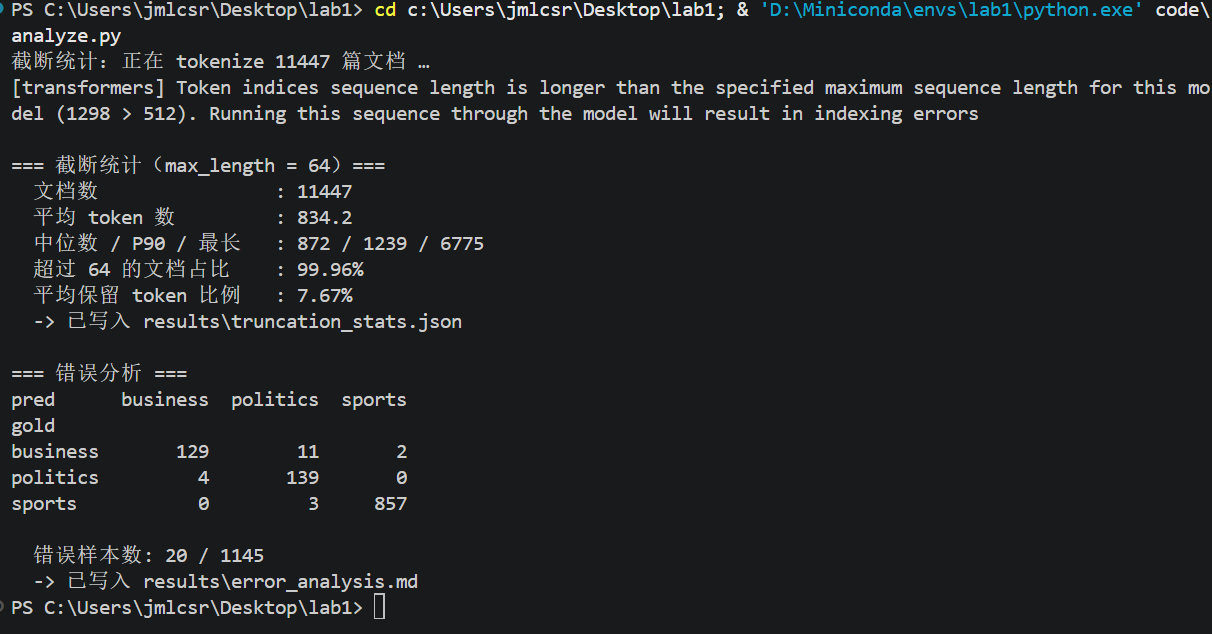
\includegraphics[width=0.95\linewidth]{t3_04_analyze.png}
  \caption{\fpath{analyze.py} 的输出：上半部分为截断统计，
  下半部分为 BERT 在测试集上的混淆矩阵与错误样本数。}
  \label{fig:analyze}
\end{figure}

\subsection{实验结果}

由于 GPU 浮点运算存在非确定性，同一配置重复运行的结果并不完全相同，
因此本节给出 \textbf{4 次独立运行}的统计结果（各次明细见表~\ref{tab:bert-runs}）。

\begin{table}[htbp]
\centering
\small
\caption{BERT 微调的 4 次独立运行结果}
\label{tab:bert-runs}
\begin{tabular}{cccccc}
\toprule
次数 & Val Macro-F1（ep1 / ep2 / ep3） & Test Acc & Test Macro-F1 \\
\midrule
1 & 0.9463 / 0.9346 / 0.9512 & 0.9843 & 0.9630 \\
2 & 0.9436 / 0.9440 / 0.9494 & 0.9817 & 0.9558 \\
3 & 0.9401 / 0.9307 / 0.9455 & 0.9843 & 0.9620 \\
4 & 0.9488 / 0.9384 / 0.9431 & 0.9825 & 0.9582 \\
\midrule
\best{均值 $\pm$ 标准差} & — & \best{0.9832 $\pm$ 0.0013} & \best{0.9597 $\pm$ 0.0033} \\
\bottomrule
\end{tabular}
\end{table}

图~\ref{fig:bert-run2}$\sim$图~\ref{fig:bert-run4} 为第 2$\sim$4 次运行的训练日志
（第 1 次的评测行见第~\ref{sec:bert-repro} 节）。

\begin{figure}[htbp]
  \centering
  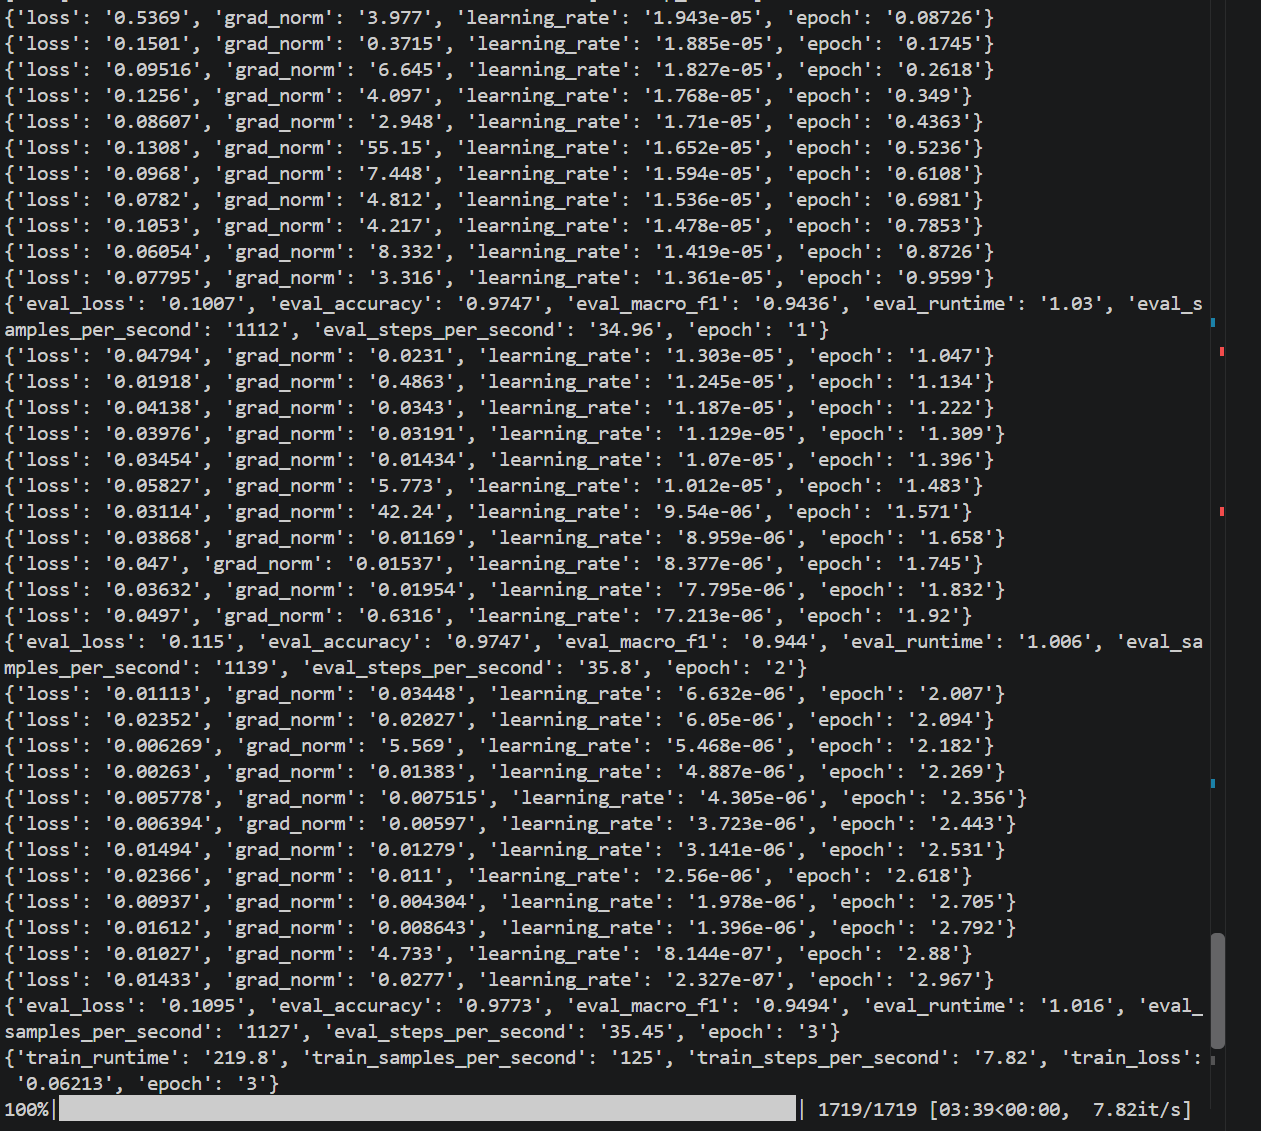
\includegraphics[width=0.95\linewidth]{t3_01_run2.png}
  \caption{BERT 第 2 次运行的训练日志。
  1,719 步，三轮 Val Macro-F1 依次为 0.9436 / 0.9440 / 0.9494。}
  \label{fig:bert-run2}
\end{figure}

\begin{figure}[htbp]
  \centering
  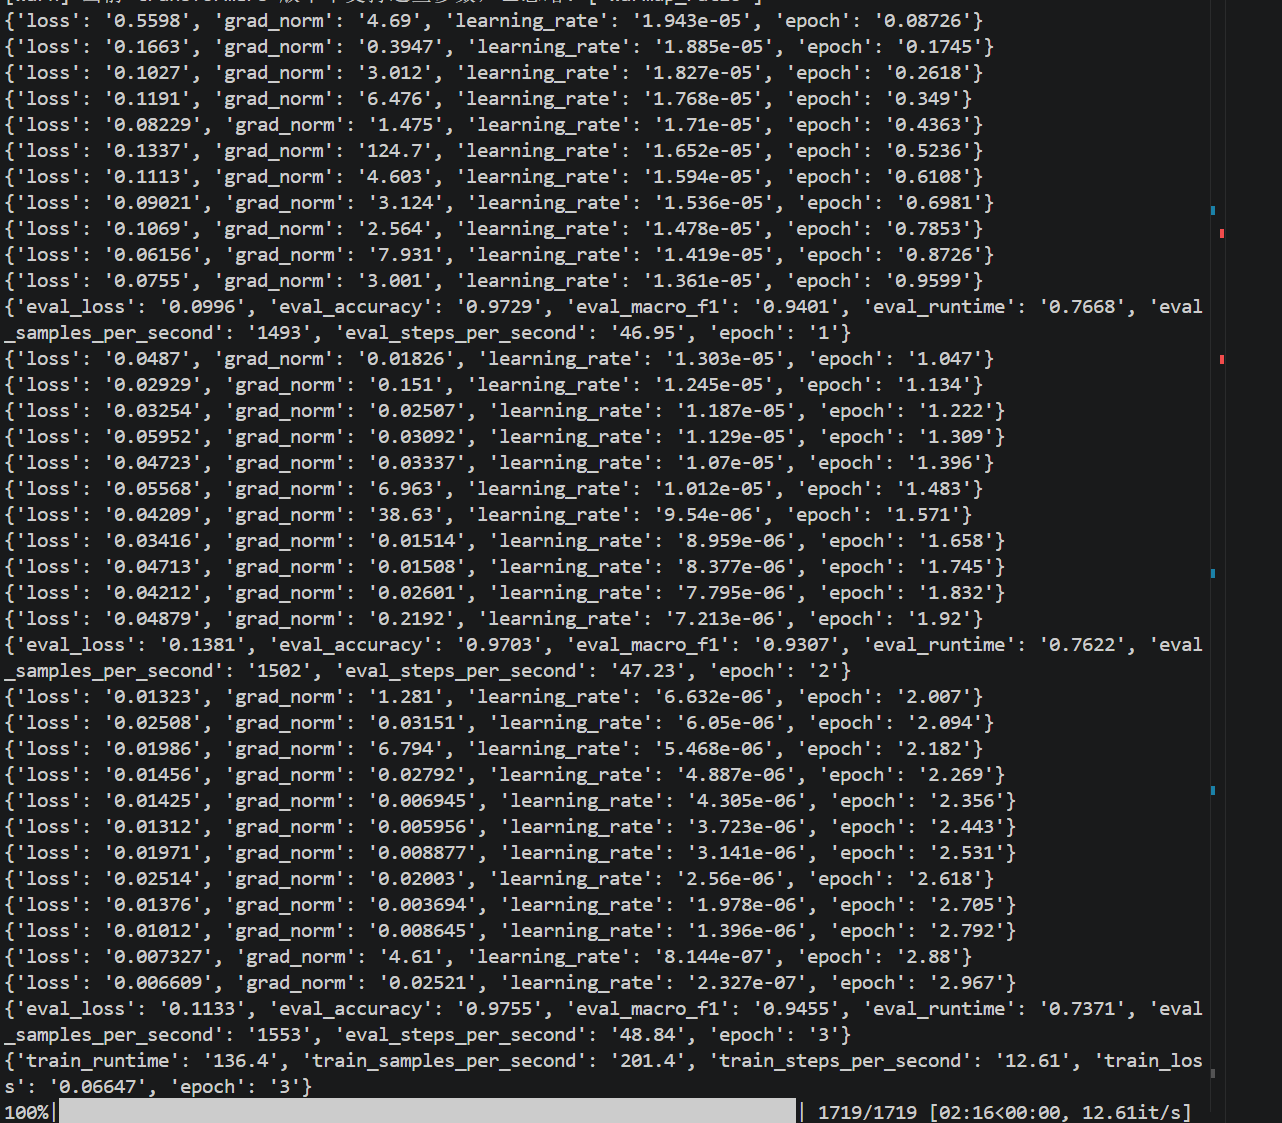
\includegraphics[width=0.95\linewidth]{t3_02_run3.png}
  \caption{BERT 第 3 次运行的训练日志。
  三轮 Val Macro-F1 依次为 0.9401 / 0.9307 / 0.9455。}
  \label{fig:bert-run3}
\end{figure}

\begin{figure}[htbp]
  \centering
  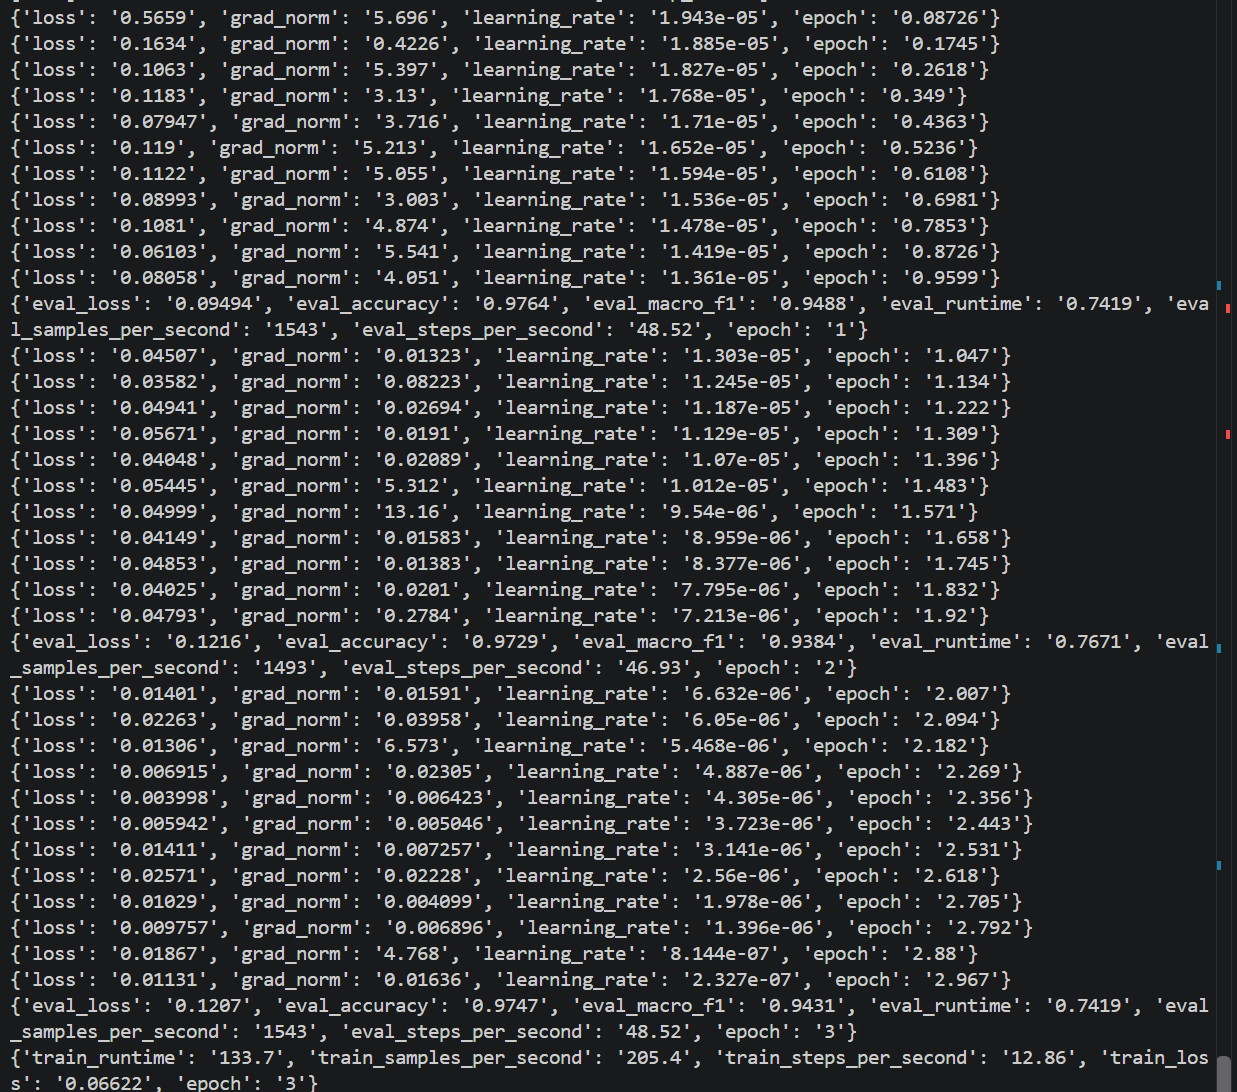
\includegraphics[width=0.95\linewidth]{t3_03_run4.png}
  \caption{BERT 第 4 次运行的训练日志。
  三轮 Val Macro-F1 依次为 0.9488 / 0.9384 / 0.9431。}
  \label{fig:bert-run4}
\end{figure}

\subsection{结果分析}

\textbf{（1）BERT 取得最优结果，但优势有限。}
4 次运行都优于最强的词袋（Word Frequency，0.9542），
平均高 \textbf{+0.0055}；但在 Accuracy 上基本持平（0.9832 vs 0.9825），
其中第 2 次运行（0.9817）甚至略低于词袋。
因此准确的表述是``\textbf{与最强词袋基线相当或略有优势}''
——``BERT 全面优于传统方法''的直觉在本任务上并不成立。

\textbf{（2）只看到 7.7\% 的内容，却拿到了最优的 Macro-F1。}
原因是这 64 个 token 对应的是\textbf{标题 + 导语}，
而新闻导语恰恰是主题信息最密集的部分。
这说明``截断''不等于``丢信息''，\textbf{关键看截掉了什么}。
但截断同时也限制了 BERT 拉开差距的空间：
它用 8\% 的内容只换来对``用满 100\% 词汇''的词袋的微弱优势。

\textbf{（3）轮间波动明显。}
例如第 1 次运行的三轮 Val Macro-F1 为 0.9463 / 0.9346 / 0.9512，
第 4 次为 0.9488 / 0.9384 / 0.9431。
epoch 1 到 2 之间时常不升反降，
与学习率在前期衰减（线性衰减调度）的过程相符。
4 次运行的末轮都接近各自最优，但\textbf{不能假设末轮总是最优}。

\subsection{多次运行与可复现性}
\label{sec:bert-repro}

\textbf{问题}：同一配置（\fpath{seed=42}）、同一数据划分，重复运行得到的指标并不相同
（Test Macro-F1 从 0.9558 到 0.9630，极差 0.0072）。

\textbf{证据}：第 1 次与第 2 次运行在\textbf{第 50 步}的 \fpath{train\_loss} 就已经不同
（0.5087 vs 0.5369）。而第 50 步之前两次运行都\textbf{没有写过任何 checkpoint}，
故该差异\textbf{不是} checkpoint 保存/回载造成的，而是训练过程本身的分歧。

第 1 次运行的三轮验证指标（节选关键字段）：

{\footnotesize
\begin{verbatim}
{'eval_loss': 0.0916, 'eval_accuracy': 0.9755, 'eval_macro_f1': 0.9463, 'epoch': '1'}
{'eval_loss': 0.1230, 'eval_accuracy': 0.9712, 'eval_macro_f1': 0.9346, 'epoch': '2'}
{'eval_loss': 0.1121, 'eval_accuracy': 0.9782, 'eval_macro_f1': 0.9512, 'epoch': '3'}
\end{verbatim}
}

\textbf{原因}：训练在 GPU 上进行，存在非确定性 kernel。
最主要的是 \fpath{nn.Embedding} 的反向传播使用 \fpath{atomicAdd}
把梯度累加到同一个词向量上（浮点加法顺序不定），
其次是 scaled\_dot\_product\_attention 的反向 kernel，
以及 bf16 下的归约顺序。
\fpath{seed=42} 只能固定\textbf{参数初始化}与\textbf{数据顺序}，
无法约束这些 kernel 的执行顺序。

\textbf{处理}：
报告 BERT 时给出均值 $\pm$ 标准差而非单次值；
结论按``相当或略有优势''表述，\textbf{不下``显著优于''的强结论}。
作为反证对照，Task 1 已实测重跑逐位一致（确定性），Task 2 的 gensim 在固定 seed 后亦稳定，
即\textbf{不确定性只出现在 GPU 上的 BERT 微调}。

% ============================================================
\section{综合对比与讨论}

\subsection{三种文本表示的横向对比}

\begin{table}[htbp]
\centering
\footnotesize
\caption{全部方法在 NYT Test Set（1145 条）上的结果汇总}
\label{tab:main}
\begin{tabular}{llccc}
\toprule
方法 & 表示类型 & 维度 & Test Accuracy & Test Macro-F1 \\
\midrule
多数类基线（全预测 sports） & — & — & 0.7511 & 0.2860 \\
\midrule
Binary BoW + LR & 二值词袋 & 53146 & 0.9790 & 0.9468 \\
Word Frequency + LR & 词频词袋 & 53146 & 0.9825 & 0.9542 \\
Binary BoW + LR（balanced） & 二值词袋 & 53146 & 0.9790 & 0.9479 \\
Word Frequency + LR（balanced） & 词频词袋 & 53146 & 0.9808 & 0.9506 \\
\midrule
GloVe-100 平均 + LR & 预训练词向量 & 100 & 0.9782 & 0.9471 \\
Word2Vec(NYT)-100 平均 + LR & 自训练词向量 & 100 & 0.9712 & 0.9308 \\
Word2Vec(AG News)-100 平均 + LR & 自训练词向量 & 100 & 0.9686 & 0.9227 \\
\midrule
\best{BERT-base-uncased} & \best{预训练语言模型微调} & \best{768} & \best{0.9832} & \best{0.9597} \\
\bottomrule
\end{tabular}
\end{table}

按 Test Macro-F1 的三层结论：

\textbf{（1）词袋在这个数据集上异常强}（0.9542）。
文本极长（平均 637 词），词袋能无损保留全部词汇信息；
而``平均词向量''把 637 词压成 100 维，信息损失巨大。
这与``词向量必然优于词袋''的常见直觉相反，
是\textbf{长文本 + 类别可分性强}这一数据特点造成的。

\textbf{（2）词向量的价值体现在``压缩比''而非``绝对性能''。}
100 维追平 53146 维，维度降低约 500 倍而性能基本不变。

\textbf{（3）只有端到端的微调才超过词袋，但优势很小}
（平均 +0.0055，约为运行波动 0.0033 的 1.7 倍）。
在长文本且类别可分性强的数据上，词袋本身就是极强的基线，
加上 BERT 被硬性限制在 64 token，它很难拉开差距。

\subsection{错误分析}
\label{sec:error}

以第 4 次运行的预测（Test Acc 0.9825）为例，错误共 \textbf{20 / 1145（1.75\%）}。

\begin{table}[htbp]
\centering
\small
\caption{BERT 测试集混淆矩阵（行 = 真实，列 = 预测）}
\label{tab:cm}
\begin{tabular}{lcccc}
\toprule
真实 $\backslash$ 预测 & business & politics & sports & 错分率 \\
\midrule
business（142） & 129 & 11 & 2 & \best{9.15\%} \\
politics（143） & 4 & 139 & 0 & 2.80\% \\
sports（860） & 0 & 3 & 857 & \best{0.35\%} \\
\bottomrule
\end{tabular}
\end{table}

由混淆矩阵可精确复原各类别指标（与 \fpath{results.json} 中的 Macro-F1 0.9582 完全一致）：

\begin{table}[htbp]
\centering
\small
\caption{由混淆矩阵计算的各类别指标（第 4 次运行）}
\label{tab:perclass}
\begin{tabular}{lccc}
\toprule
类别 & Precision & Recall & F1 \\
\midrule
business & 0.9699 & 0.9085 & 0.9382 \\
politics & 0.9085 & 0.9720 & 0.9392 \\
sports & 0.9977 & 0.9965 & 0.9971 \\
\midrule
Macro 平均 & 0.9587 & 0.9590 & \best{0.9582} \\
\bottomrule
\end{tabular}
\end{table}

错误分布高度集中：

\begin{table}[htbp]
\centering
\small
\caption{错误样本的类别对分布}
\label{tab:errdist}
\begin{tabular}{lcc}
\toprule
真实 $\to$ 预测 & 次数 & 占全部错误 \\
\midrule
\best{business $\to$ politics} & 11 & 55\% \\
politics $\to$ business & 4 & 20\% \\
sports $\to$ politics & 3 & 15\% \\
business $\to$ sports & 2 & 10\% \\
\bottomrule
\end{tabular}
\end{table}

\textbf{结论：}

\textbf{（1）错误集中在 business $\leftrightarrow$ politics（15/20 = 75\%）。}
两类都是``社会经济/公共事务''题材，边界天然模糊。
典型错例：\emph{``this spring, the missouri chamber of commerce urged the state
legislature to accept the federal government's plan to expand medicaid for the poor
and disabled. the business lobbying group had not suddenly gone rogue.''}
——\textbf{商业团体在做政治游说}，被判定为 politics 并不难理解。

\textbf{（2）sports 几乎不会错}（错分率 0.35\%，3/860）。
该类的判别特征极强，也是它支撑起 0.98 Accuracy 的原因。

\textbf{（3）错误方向不对称}：business $\to$ politics 有 11 次，反向仅 4 次。
business 报道常涉及政策与政府，更容易被``政治化''。

\textbf{（4）存在标注歧义的可能。}
错例中包含\emph{``the departure of chairman ben s. bernanke of the federal reserve''}、
\emph{``the costs of the 16-day partial government shutdown''}等本身横跨政治与经济的报道，
人工标注也有争议空间。

\textbf{（5）Accuracy 的钝感。}
sports 占 75.1\%，即使把 13 个 business 错例全部修正，Accuracy 也只提升约 0.011。
这再次说明在该数据集上\textbf{Macro-F1 比 Accuracy 更有区分度}。

\subsection{结论与局限性}

\textbf{主要结论}

\begin{enumerate}
  \item 在 NYT 三分类任务上，\textbf{词袋表示是一个极强的基线}，
        Word Frequency + LR 即可达到 0.9542 的 Macro-F1；
  \item \textbf{词向量平均的主要贡献是维度压缩}（约 500 倍）而非绝对性能提升，
        且其性能与词覆盖率完全同序；
  \item \textbf{BERT 微调取得最优 Macro-F1（$0.9597\pm0.0033$），
        但相对词袋的优势很小}（平均 +0.0055），且单次结果不可复现；
  \item 错误集中在语义边界模糊的类对（business $\leftrightarrow$ politics），
        而多数类 sports 几乎不会错。
\end{enumerate}

\textbf{局限性}

\begin{itemize}
  \item \textbf{文档向量取平均丢失了语序}，这是 Task 2 性能受限的重要内因；
  \item \textbf{BERT 受 64 token 截断限制}，只使用约 7.7\% 的文本，
        若能放宽长度（如 256），其优势可能更明显；
  \item \textbf{GPU 非确定性}使得 BERT 的结果需以多次运行的均值表述，
        本次仅运行 4 次，标准差估计本身也不够稳定；
  \item 受算力限制，未进行超参数搜索（学习率、batch size、warmup 均取常用默认值），
        \fpath{warmup\_ratio} 因所用 transformers 版本不支持而被忽略。
\end{itemize}

% ============================================================
\appendix

\section{运行环境与复现步骤}

完整代码与运行说明见仓库根目录的 \fpath{README.md}，
本实验记录见 \fpath{results/实验记录.md}，机器可读指标见 \fpath{results/results.json}。
主要运行顺序如下（需先安装依赖并下载 nltk 分词数据与 GloVe 词向量）：

{\small
\begin{verbatim}
# Step 0：统一数据划分（80/10/10，seed=42）
python code/step0_split.py --stratify

# Task 1：两种词袋表示
python code/task1_bow.py --mode binary
python code/task1_bow.py --mode freq

# Task 2：三组词向量实验
python code/task2_word2vec.py --source glove --glove embeddings/glove.6B.100d.txt
python code/task2_word2vec.py --source ag
python code/task2_word2vec.py --source nyt

# Task 3：BERT 微调（3 epochs）
python code/task3_bert.py --no_save --epochs 3

# 收尾分析：截断统计 + 错误分析
python code/analyze.py
\end{verbatim}
}

其中 \fpath{--no\_save} 表示不保存 checkpoint、训练结束后不回载``最佳模型''。
这样处理有两个目的：一是使最终评测严格对应\textbf{第 3 轮结束时的模型}，
与作业``训练 3 epochs''的要求严格对应；
二是规避 transformers 5.19 在 \fpath{save\_pretrained} $\to$ \fpath{load\_state\_dict}
往返中 LayerNorm 参数命名不一致（存为 \fpath{gamma}/\fpath{beta}、
读取时期望 \fpath{weight}/\fpath{bias}）所产生的大量警告（详见附录~\ref{app:debug}）。

\section{问题排查记录}
\label{app:debug}

本节记录实现过程中遇到并定位的四个问题，其中第 4 条是一个由自己引入的真实 bug。

\textbf{（1）sklearn 版本变化导致的参数失效警告。}
训练 Task 1 时 sklearn 1.9 报出
\fpath{FutureWarning: 'n\_jobs' has no effect since 1.8 and will be removed in 1.10}
（见图~\ref{fig:njobs}）。该参数在新版本已被忽略，
为保持输出干净并避免未来版本报错，已将其移除；
移除后重跑结果逐位一致，反过来也验证了 Task 1 的确定性。

\begin{figure}[htbp]
  \centering
  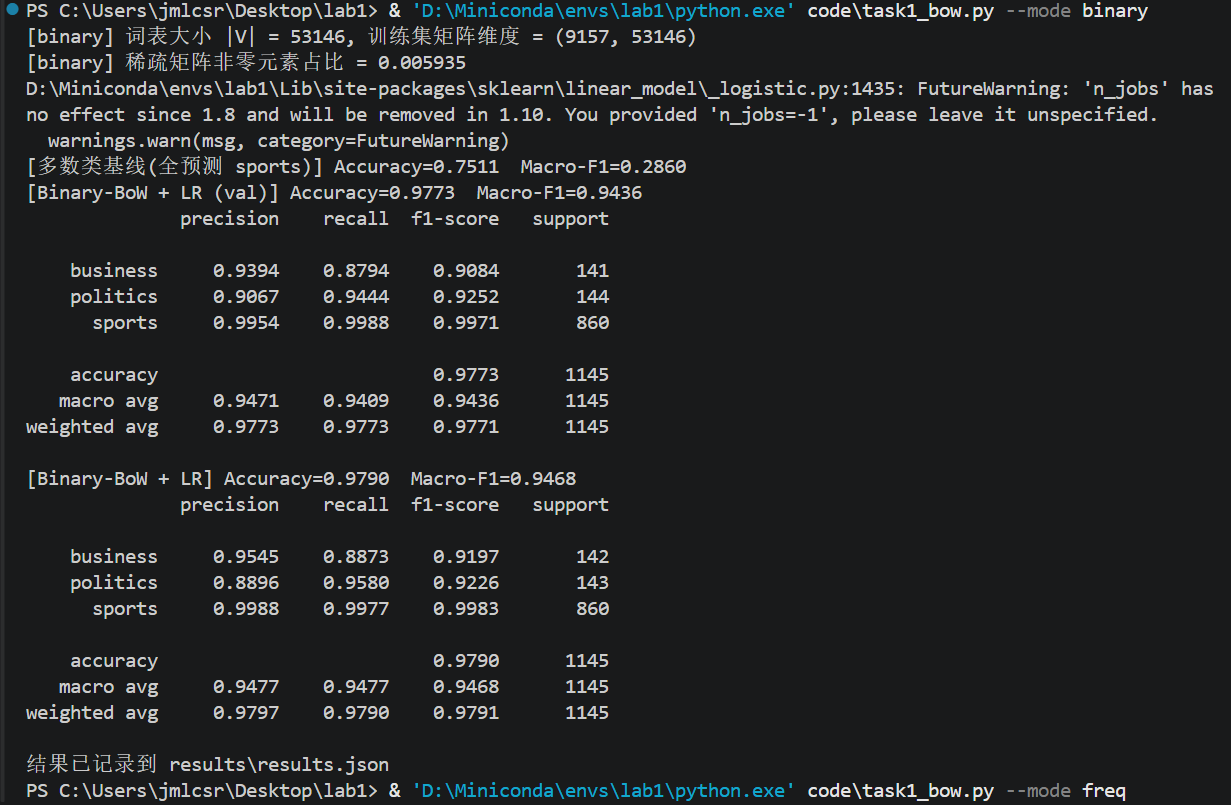
\includegraphics[width=0.95\linewidth]{t1_02_binary_njobs_warning.png}
  \caption{Binary BoW 运行时 sklearn 打印的 \fpath{n\_jobs} 参数失效警告，
  其后为 Word Frequency 的运行命令。该参数随后被移除。}
  \label{fig:njobs}
\end{figure}

\textbf{（2）transformers 5.19 的参数改名与不支持。}
\fpath{TrainingArguments} 中 \fpath{evaluation\_strategy} 已在 4.46 改名为 \fpath{eval\_strategy}；
\fpath{warmup\_ratio} 在当前版本不被支持。
脚本通过 \fpath{inspect.signature} 动态检查可用参数名，
自动选择正确的名字并过滤掉不支持的参数（运行时会打印
\fpath{[warn] 当前 transformers 版本不支持这些参数，已忽略: ['warmup\_ratio']}），
因此实际训练未使用 warmup。

\textbf{（3）LayerNorm 参数在保存/加载往返中的键不匹配。}
不使用 \fpath{--no\_save} 时，训练结束回载最佳 checkpoint 会打印约 50 个键的
\fpath{missing}/\fpath{unexpected} 警告：
保存的键名是 \fpath{...LayerNorm.gamma}/\fpath{beta}，
而加载时期望 \fpath{...LayerNorm.weight}/\fpath{bias}。
为确认其是否影响结果，对比了回载前后的验证指标：

{\footnotesize
\begin{verbatim}
回载前（训练中评测）: eval_loss 0.1121      eval_accuracy 0.9782  eval_macro_f1 0.9512
回载后（trainer.evaluate）: eval_loss 0.11212880...  eval_accuracy 0.97816593...
                            eval_macro_f1 0.95117597...
\end{verbatim}
}

两者逐位一致，说明该警告\textbf{不影响最终结果}，属于命名往返问题。
正式实验改用 \fpath{--no\_save} 后该路径不再触发。

\textbf{（4）一个真实的 bug：报错点在 collator，根因在数据构造。}
加入 \fpath{--no\_save} 选项后，训练在第一步即抛出：

\begin{verbatim}
TypeError: vars() argument must have __dict__ attribute
  (transformers/data/data_collator.py:126)
\end{verbatim}

最初怀疑是 collator 被框架重复包装，但在换成自定义 collator 后，
报错变成 \fpath{AttributeError: 'TextClfDataset' object has no attribute 'keys'}——
两次报错都指向 ``\fpath{collate\_fn} 收到的第一个元素就是数据集对象本身''。
据此回看数据构造代码，发现该行末尾多了一个逗号：

\begin{verbatim}
ds_train = TextClfDataset(train_df["text"], y_tr, tokenizer), args.no_save
\end{verbatim}

尾随逗号使右值成为 \textbf{tuple}，torch 便把该 tuple 当作``数据集''：
其长度为 2，\fpath{ds[0]} 恰好是那个 \fpath{TextClfDataset} 对象，
于是 \fpath{collate\_fn} 收到 \fpath{[Dataset]}，
默认 collator 的 \fpath{vars(f)} 与自定义 collator 的 \fpath{f.keys()} 相继失败。
\textbf{修正该行后，\fpath{--no\_save} 连续 3 次稳定运行成功}。
这里的体会是： AI 大规模改动代码时容易在不经意处引入小错误，
而这类错误让 AI 反复推理往往定位不到，
最终是靠让它把相关代码完整遍历一遍发现了根因。

\vspace{6pt}
\noindent
\textbf{附：GloVe 词向量获取过程中的网络问题。}
官方地址 \fpath{http://nlp.stanford.edu/data/}\allowbreak\fpath{glove.6B.zip}（约 822\,MB）在国内直连被限速到约 12\,KB/s；
改用 Python 经系统代理访问镜像后成功下载（331\,MiB，约 1 分钟，$\sim$5.3\,MB/s）。
经验：换源前必须核对文件大小（正确为 347,117,594 字节，
某些镜像提供的是仅 134\,MB 的裁剪版本）；
且 Windows 自带的 \fpath{curl.exe} 不读取系统代理，而 Python 的 \fpath{urllib} 会读取。

\end{document}
